% coding:utf-8

\section{Digitally-Controlled Oscillator}

\subsection{Übersicht}
\begin{frame}
    \frametitle{}
    \framesubtitle{}
      \begin{figure}
        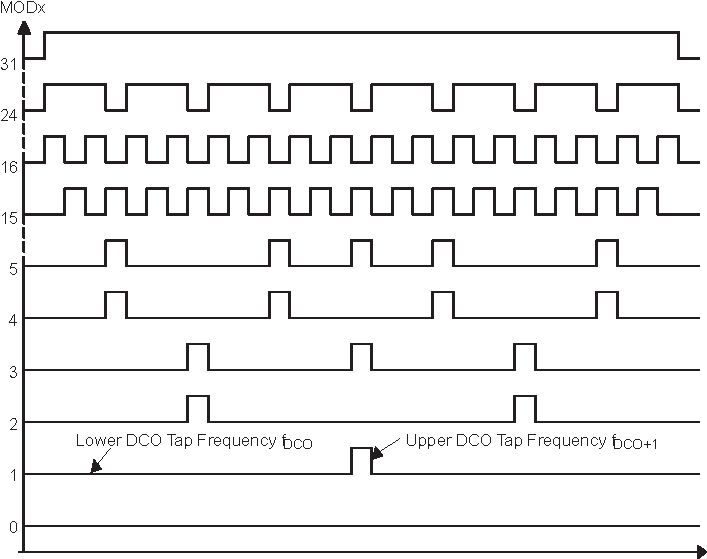
\includegraphics[width=0.7\columnwidth]{fig/ti_fg_dco_mod.pdf}
        \caption{Funktionsweise Modulation}
      \end{figure}
\end{frame}

\subsection{Modulation}
\begin{frame}
  \begin{tikztimingtable}
    \mbox{\uncover<+->{MOD =  0}} & <.->33L<*>\\
    \mbox{\uncover<+->{MOD =  1}} & <.->16LH16L<*>\\
    \mbox{\uncover<+->{MOD =  2}} & <.->8LH15LH8L<*>\\
    \mbox{\uncover<+->{MOD =  3}} & <.->8L2{H7L}H8L<*>\\
    \mbox{\uncover<+->{MOD = 16}} & <.->L16{HL}<*>\\
    \mbox{\uncover<+->{MOD = 24}} & <.->L8{3HL}<*>\\
    \mbox{\uncover<+->{MOD = 31}} & <.->L31HL<*>\\
  \end{tikztimingtable}
\end{frame}